\documentclass{standalone}
\usepackage{pgfplots}
\pgfplotsset{compat=1.17}

\begin{document}

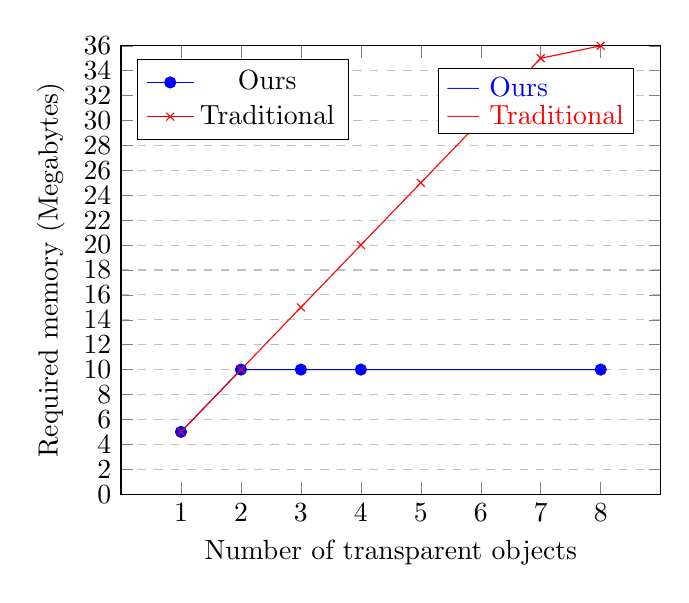
\begin{tikzpicture}
\begin{axis}[
    xlabel={Number of transparent objects},
    ylabel={Required memory (Megabytes)},
    xmin=0, xmax=9,
    ymin=0, ymax=36,
    xtick={1,2,3,4,5,6,7,8},
    ytick={0,2,...,36},
    legend pos=north west,
    ymajorgrids=true,
    grid style=dashed,
]

\addplot[
    color=blue,
    mark=*,
    ]
    coordinates {
        (1,5)(2,10)(3,10)(4,10)(8,10)
    };
    \addlegendentry{Ours}
    
\addplot[
    color=red,
    mark=x,
    ]
    coordinates {
        (1,5)(2,10)(3,15)(4,20)(5,25)(6,30)(7,35)(8,36)
    };
    \addlegendentry{Traditional}

\end{axis}

% Customize the legend's appearance to match the image
\node[draw,fill=white,anchor=north east] at (rel axis cs: 0.95,0.95) {\shortstack[l]{
    \textcolor{blue}{\textbf{---} Ours} \\ 
    \textcolor{red}{\textbf{---} Traditional}
}};

\end{tikzpicture}

\end{document}